\documentclass[twoside, 11pt]{article}
\usepackage{../estilo-apuntes}
%\usepackage{amsmath,amssymb}
%\usepackage[utf8]{inputenc}
%\usepackage[spanish]{babel}
%\usepackage{caption}
%\usepackage[]{graphicx}
%\usepackage{enumerate}
%\usepackage{amsthm}
%\usepackage{tikz-cd}
%\usetikzlibrary{babel}
%\usepackage{pgf,tikz}
%\usepackage{mathrsfs}
%\usepackage{bm}  
%\usetikzlibrary{arrows}
%\usetikzlibrary{cd}
%\usepackage[spanish]{babel}
%\usepackage{fancyhdr}
%\usepackage{titlesec}
%\usepackage{floatrow}
%\usepackage{makeidx}
%\usepackage[tocflat]{tocstyle}
%\usetocstyle{standard}
%\usepackage{subfiles}
%\usepackage{color}  
%\usepackage{hyperref}
%\hypersetup{colorlinks=true,citecolor=red, linkcolor=blue}
%\usepackage{eurosym}
%%\usepackage{ntheorem}
%
%
%\renewcommand{\baselinestretch}{1,4}
%\setlength{\oddsidemargin}{0.25in}
%\setlength{\evensidemargin}{0.25in}
%\setlength{\textwidth}{6in}
%\setlength{\topmargin}{0.1in}
%\setlength{\headheight}{0.1in}
%\setlength{\headsep}{0.1in}
%\setlength{\textheight}{8in}
%\setlength{\footskip}{0.75in}
%
%\theoremstyle{definition}
%
%\newtheorem{teorema}{Teorema}[section]
%\newtheorem{defi}[teorema]{Definición}
%\newtheorem{coro}[teorema]{Corolario}
%\newtheorem{lemma}[teorema]{Lema}
%\newtheorem{ej}[teorema]{Ejemplo}
%\newtheorem{ejs}[teorema]{Ejemplos}
%\newtheorem{observacion}[teorema]{Observación}
%\newtheorem{observaciones}[teorema]{Observaciones}
%\newtheorem{prop}[teorema]{Proposición}
%\newtheorem{propi}[teorema]{Propiedades}
%\newtheorem{nota}[teorema]{Nota}
%\newtheorem{notas}[teorema]{Notas}
%\newtheorem*{dem}{Demostración}
%\newtheorem{ejer}[teorema]{Ejercicio}
%\newtheorem{problem}[teorema]{Problema}
%\newtheorem{concl}[teorema]{Conclusión}
%
%\providecommand{\abs}[1]{\lvert#1\rvert}
%\providecommand{\sen}[1]{sen #1}
%\providecommand{\norm}[1]{\lVert#1\rVert}
%\providecommand{\ninf}[1]{\norm{#1}_\infty}
%\providecommand{\numn}[1]{\norm{#1}_1}
%\providecommand{\gabs}[1]{\left|{#1}\right|}
%\newcommand{\bor}[1]{\mathcal{B}(#1)}
%\newcommand{\R}{\mathbb{R}}
%\newcommand{\Z}{\mathbb{Z}}
%\newcommand{\N}{\mathbb{N}}
%\newcommand{\Q}{\mathbb{Q}}
%\newcommand{\C}{\mathbb{C}}
\newcommand{\LL}{\mathcal{L}}
%\newcommand{\Tau}{\mathcal{T}}
%\newcommand{\verteq}{\rotatebox{90}{$\,=$}}
%\newcommand{\vertequiv}{\rotatebox{110}{$\,\equiv$}}
%\providecommand{\lrg}{\longrightarrow}
%\providecommand{\func}[2]{\colon{#1}\longrightarrow{#2}}
%\newcommand*{\QED}{\hfill\ensuremath{\blacksquare}}
%\newcommand*\circled[1]{\tikz[baseline=(char.base)]{
%            \node[shape=circle,draw,inner sep=1.5pt] (char) {#1};}}
%\newcommand*{\longhookarrow}{\ensuremath{\lhook\joinrel\relbar\joinrel\rightarrow}}


\begin{document}
%\title{Topología de Superficies}
%\author{Antonio Rafael Quintero Toscano\\ Javier Aguilar Martín}
%\date{Curso 2016/2017}
%\maketitle

\author{Javier Aguilar Martín }
\date{\today}
\title{La conjetura de Smale:\\ $Diff(S^3)\simeq O(4)$}

\maketitle


\begin{abstract}
Un guion que no pretende ser totalmente detallado ni riguroso sobre la prueba de Hatcher de la conjetura de Smale. RECUERDA PONER LAS DOS COSAS COMO BIBLIOGRAFÍA
\end{abstract}


	\vfill
	Esta obra está licenciada bajo la Licencia Creative Commons Atribución 3.0 España. Para ver una copia de esta licencia, visite \url{http://creativecommons.org/licenses/by/3.0/es/} o envíe una carta a Creative Commons, PO Box 1866, Mountain View, CA 94042, USA.


\newpage
\tableofcontents

\newpage

\section{Introducción y enunciado equivalente}
\subsection{Introducción}


\subsection{Enunciados equivalentes}\label{equivalentes}
Es conocido que $Diff(S^n)\simeq O(n+1)\times Diff(D^n\ rel\ \partial D^n)$ para todo $n$. Por tanto, la conjetura de Smale $Diff(S^4)\simeq O(4)$ es equivalente a $Diff(D^3\ rel\ \partial D^3)\simeq *$. El teorema puede ser reenunciado como como que para los espacios de smooth embeddings $Emb(D^3,\R^3)$ y $Emb(S^2,\R^n)$, la restricción $\rho:Emb(D^3,\R^3)\to Emb(S^2,\R^n)$ induce sobreyección en $\pi_k$ para todo $k$, pues $\rho$ es una fibración cuyas fibra es precisamente $Diff(D^3\ rel\ \partial D^3)$ (se usa la sucesión exacta larga de homotopía de una fibración). Consideremos ahora el diagrama
\[
\begin{tikzcd}
Emb(D^3,\R^3)\arrow[rr, "\rho"] \arrow[dr, "\simeq"]& & Emb(S^2,\R^n)\arrow[dl]\\
&GL(n,\R)&
\end{tikzcd}
\]
donde la equivalencia de homotopía consiste en evaluar la derivada en un punto. A partir de esto podemos enunciar equivalentemente el teorema como ``el espacio de smoothly embedded 2-esferas en $\R^3$ es contráctil''. Este espacio es el espacio de órbitas $Emb(S^2,\R^3)/Diff(S^2)$. Como $Diff(S^2)\simeq O(3)$, la contractibilidad del espacio es equivalente a que $\rho$ sea equivalencia de homotopía, pues $GL(n,\R)\simeq O(n)$ mediante Gram-Schmidt. Esta última versión será la que se probará.


\section{Normalización, partición de la unidad y cirugía}
\subsection{Normalización}
\begin{defi}
Una superficie orientada $S$ de $\R^3$ se dice \emph{elemental} si verifica las siguientes condiciones:
\begin{enumerate}
\item Cada curva del borde está en un plano horizontal, siendo $S$ vertical en un entorno de cada curva. 
\item La intersección de $S$ con una línea vertical es conexa (posiblemente vacía).
\item Si denotamos por $S^+$ (respectivamente $S^-$) a la adherencia del conjunto de puntos donde la normal tiene coordenaza $z$ estrictamente positiva (respectivamente negativa), $S^+$ y $S^-$ están aisladas la una de la otra. 
\end{enumerate}
\end{defi}

\begin{prop}[de normalización]
Dada una familia de esferas $\Sigma_t$, $t\in S^k$, existe un recubrimiento de $S^k$ por bolas abiertas $B_i$, existen planos horizontales $P_{ij}$ (todos distintos) y una deformación de $\Sigma_t$ a una familia $\Sigma'_t$ tal que:
\begin{enumerate}
\item Para todo $t\in B_i$ y para todo $j$, la parte de $\Sigma'_t$ comprendida entre $P_{ij}$ y $P_{ij+1}$ es una superficie elemental
\item $\Sigma'_t$ es la unión de las partes anteriores. 
\end{enumerate}
\end{prop}
\begin{dem}
Sea $U_i^{\pm}\subseteq\Sigma_t$ el conjunto de puntos donde la normal exterior forma un ángulo $\leq\frac{\pi}{4}$ con el vector $\pm(0,0,1)$. Sea $\rho_t:\Sigma_t\to [0,1]$ una familia de funciones con soporte en $U_i^+\cup U_i^-$ con $\rho_t>0$ en los puntos que tienen plano tangente horizontal. Definimos el campo de vectores $v_t$ sobre $\Sigma_t$ como $grad(h_t)+\rho_t\cdot(0,0,1)$, donde $h_t$ es la función altura de $\Sigma_t$. Por definición, $v_t$ tiene coordenada $z$ positiva en $\Sigma_t$ y puede ser extendido a un campo de vectores en $\R^3$ con la misma propiedad. Sea $f_t$ una familia de difeomorfismos que preserven la altura en $\R^3$ llevando las trayectorias de $v_t$ a líneas verticales de $\R^3$. 

Existe $\delta\geq 0$, independiente de $t$, tal que todo segmento vertical en $\R^3$ de longitud menor o igual que $\delta$ interseca con $\Sigma'_t=f_t(\Sigma_t)$ en un conjunto conexo. Esto se sigue porque el campo de vectores $(0,0,1)$ sobre $\Sigma'_t$ solo puede apuntar a un lado de $\Sigma'_t$ localmente. Esto es, $(0,0,1)$ apunta hacia fuera en $f_t(U_i^+)$ y hacia dentro en $f_t(U_i^-)$, estando estos conjuntos separados por una distancia $d>0$ independiente de $t$. Podemos suponer que $\delta<\frac{1}{2}d$. 

Para cada $t$ podemos elegir un número finito de planos horizontales $P_{ij}$ transversales a $\Sigma'_t$ de modo que planos adyacentes estén a distancia estrictamente menor que $\delta$ y que $\Sigma'_t$ se encuentre entre los $P_{ij}$ extremos. Estos planos se mantienen transversales a $\Sigma'_t$ en alguna bola abierta $B_i\subseteq S^k$. Por compacidad de $S^k$, podemos recubir $S^k$ con un número finito de estas bolas. Podemos suponer que los $P_{ij}$ son distintos sin problema pues se escogen de un conjunto abierto de planos horizontales. 

Por construcción, para cada $i$ y $t\in B_i$, la parte de $\Sigma'_t$ entre planos adyacentes son superficies elementales ya que hemos tomado $\delta<\frac{1}{2}d$ y $\Sigma'_t$ es la unión de estas superficies
\QED
\end{dem}

A partir de ahora nos referiremos a $\Sigma'_t$ como $\Sigma_t$. 

\subsection{Función de Hatcher}
Sea $C_t$ la unión de las curvas $\Sigma_t\cap P_{ij}$ y $C=\bigcup_t C_t$. La unión $C$ tiene una topología natural: podemos seguir continuamente la deformación de $c_t$, componente de $\Sigma_t\cap P_{ij}$, a medida que $t$ recorre $B_i$. Podemos definir un orden parcial $c_t>c'_t$ si $c_t$ y $c'_t$ están en el mismo $P_{ij}$ y $c_t$ rodea a $c'_t$. 

\begin{prop}
Existe una función (de Hatcher) $\lambda:\pi_0(C)\to (0,1)$ inyectiva y monónota decreciente, es decir, $c_t>c'_t$ implica $\lambda(c_t)<\lambda(c'_t)$.
\end{prop}
\begin{dem}
Para cada $t$ fijo podemos asociar un grafo a los $c_t$ como en la siguiente figura.

\begin{tikzpicture}[line cap=round,line join=round,>=triangle 45,x=1.0cm,y=1.0cm]
\clip(-3,1) rectangle (9,6);
\draw [rotate around={1.1457628381751033:(0.,3.7)},line width=2.pt] (0.,3.7) ellipse (2.974204220404773cm and 2.2009749532135885cm);
\draw [line width=2.pt] (-2.,3.66) circle (0.6811754546370558cm);
\draw [line width=2.pt] (0.66,3.98) circle (1.3613228860193307cm);
\draw [line width=2.pt] (0.66,3.98) circle (0.6276941930590085cm);
\draw [line width=2.pt] (7.04,5.6)-- (5.7,4.12);
\draw [line width=2.pt] (7.04,5.6)-- (8.32,4.04);
\draw [line width=2.pt] (8.32,4.04)-- (8.32,2.54);
\begin{scriptsize}
\draw [fill=black] (7.04,5.6) circle (2.5pt);
\draw [fill=black] (5.7,4.12) circle (2.5pt);
\draw [fill=black] (8.32,4.04) circle (2.5pt);
\draw [fill=black] (8.32,2.54) circle (2.5pt);
\end{scriptsize}
\end{tikzpicture}

El grafo se mantiene isomorfo en toda la bola $B_i\ni t$, teniendo siempre una cantidad finita de vértices, y como hay una cantidad finita de bolas, podemos construir la función asignando valores del intervalo $(0,1)$ a los vértices.
\QED
\end{dem}
\subsection{Partición de la unidad}
Elegimos $\varepsilon>0$ tal que para $c_t\neq c'_t$ se tiene $|\lambda(c_t)-\lambda(c'_t)|>2\varepsilon$, y $\delta>0$ tal que dos planos $P_{ij}$ distan de al menos $2\delta$ y que $\Sigma_t$ sea vertical en un $\delta$-entorno de $P_{ij}$. Sean $\Gamma_i=\{(t,\lambda(c_t))\in B_i\times (0,1)\}$ y $\widetilde{\Gamma}_i$ un $\varepsilon$-entorno de $\Gamma_i$. Para cada $i$, se define $T_i\cong S^{k-1}\times[0,1]\subset S^k\times[0,1]$ como como un anillo que une $\partial B_i\times\{1\}$ con $\partial B'_i\times\{0\}$, siendo $B'_i$ bolas abiertas contenidas en las $B_i$ y que recubren $S^k$. Cada $\widetilde{\Gamma}_i\cap T_i$ es una unión de subanillos cuyas proyecciones sobre $S^k$ denotamos $Z_{il}$. Denotamos $E_i$ a $\widetilde{\Gamma}_i$ truncado por $B'_i$, unión de bandas tal como muestra la siguiente figura.

\definecolor{qqqqff}{rgb}{0.,0.,1.}
\definecolor{ffqqqq}{rgb}{1.,0.,0.}
\definecolor{uququq}{rgb}{0.25098039215686274,0.25098039215686274,0.25098039215686274}
\begin{center}

\begin{tikzpicture}[line cap=round,line join=round,>=triangle 45,x=1.0cm,y=1.0cm]
\clip(-1,-0.1) rectangle (6,5.5);
\draw[line width=2.pt,color=uququq,fill=uququq,fill opacity=0.10000000149011612] (2.,5.) -- (2.36,5.) -- (2.34,0.) -- (2.,0.) -- cycle;
\draw [line width=2.pt] (0.,0.)-- (0.,5.);
\draw [line width=2.pt] (0.,5.)-- (5.,5.);
\draw [line width=2.pt] (5.,5.)-- (5.,0.);
\draw [line width=2.pt] (5.,0.)-- (0.,0.);
\draw [line width=2.pt] (0.,3.72)-- (5.,5.);
\draw [line width=2.pt] (0.,1.)-- (5.,0.);
\draw [line width=2.pt] (2.,5.)-- (2.,0.);
\draw [line width=2.pt] (2.36,5.)-- (2.34,0.);
\draw [line width=2.pt,color=uququq] (2.,5.)-- (2.36,5.);
\draw [line width=2.pt,color=uququq] (2.36,5.)-- (2.34,0.);
\draw [line width=2.pt,color=uququq] (2.34,0.)-- (2.,0.);
\draw [line width=2.pt,color=uququq] (2.,0.)-- (2.,5.);
\draw [line width=2.pt,dash pattern=on 4pt off 4pt] (2.,4.232)-- (0.,4.128125);
\draw [line width=2.pt,dash pattern=on 4pt off 4pt] (2.357293868921776,4.323467230443974)-- (0.,4.3);
\draw [line width=2.8pt,,color=ffqqqq] (0.,4.3)-- (0.,4.128125);
\draw [line width=2.8pt,,color=qqqqff] (0.,3.72)-- (0.,1.);
\draw [color=qqqqff](-0.7,2.8156250000000003) node[anchor=north west] {$B_i'$};
\draw [color=ffqqqq](-0.7,4.534375) node[anchor=north west] {$Z_{il}$};
\draw (-0.7,5.08125) node[anchor=north west] {$B_i$};
\draw [line width=2.pt,dotted] (2.1568749999999994,5.)-- (2.1725,0.);
\draw (1.9,5.628125) node[anchor=north west] {$\tilde{\Gamma}_i$};
\end{tikzpicture}
\end{center}

Podemos decir que $E=\bigcup E_i$ juega el papel de una partición de la unidad, pues $\partial E$ induce una partición de $t\times [0,1]$ variando continuamente con $t$. Sea $X_i$ la proyección sobre $S^k$ de $\Gamma_i\cap T_i$; $X_i=\bigcup X_{il}$, donde $X_{il}$ es el alma de $Z_{il}\cong X_{il}\times [-1,1]$. La coordenada transversal $t_{il}$ crece en el sentido que va de $B'_i$ a $B_i$. 

Nótese que, para $i$ fijo, los $Z_{il}$ son disjuntos dos a dos por el $\varepsilon$ que se ha elegido. Se tomará un recubrimiento $\{B_i\}$ tal que cada $t$ pertenezca a lo sumo a $k+1$ bolas. Se puedeN elegir los $B'_i$ de forma que la unión de los $t$ que pertenece exactamente a $q$ $Z_{il}$, $1\leq q\leq k$, sea una unión disjunta de \emph{cubos} que tengan por alma una componente de la intersección de $q$ $X_{il}$, con los $t_{il}$ respectivas como coordenadas transversales, y que ningún $t$ pertenezca a $k+1$ $Z_{il}$. 

\subsection{Cirugía}
Para cada $t$ fijo, construimos los objetos $\Sigma_{tu}$. Los valores $\lambda(c_t)$ se ordenan en $u^1=\lambda(c_t^1)>u^2=\lambda(c_t^2)>\cdots$. Sea $\Delta(c_t)$ el disco horizontal bordeado por $c_t$. Para $u>u^1$, $\Sigma_{tu}=\Sigma_t$. Para $u=u^1$, $\Sigma_{tu}=\Sigma_t\cup \Delta(c_t^1)$ (aparición de un disco de cirugía). Si $u\in[u^1, u^1-\varepsilon]$, ejecutamos la cirugía: $\Delta(c_t^1)$ es reemplazado por dos discos $\Delta^+$ y $\Delta^-$ que se separan progresivamente, uno hacia arriba y otro hacia abajo hasta una distancia de $\Delta(c_t^1)$ igual a $\lambda(c_t)\cdot\delta$; al mismo tiempo retiramos el anillo vertical entre $\partial\Delta^+$ y $\partial\Delta^-$. Después de esto no añadimos ninguna cirugía hasta $u=u^2$ y repetimos. 

\begin{figure}[h!]
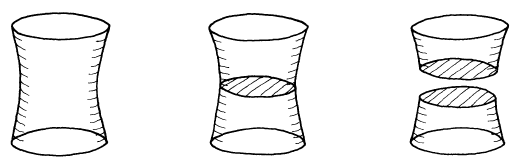
\includegraphics[scale=0.6]{cirugia}
\end{figure}

Hay una manera de describir $\Sigma_{tu}$ de modo único como unión de esferas que tienen solamente un disco horizontal en común dos a dos. Cada una de ellas es un \emph{factor} y sus discos horizontales se llaman \emph{caras}. Una esfera que es unión de superficies elementales con discos horizontales se dice \emph{primitiva}. Cada componente de $\Sigma_{t0}$ es una esfera primitiva a la que se le han añadido discos de cirugía. Si $\Delta$ es una cara común a dos factores $\Sigma_1$ y $\Sigma_2$, se dice que $\Delta$ es una cara \emph{suma} si $\overline{\Sigma}_1$ y $\overline{\Sigma}_2$ son bolas que intersecan solo en $\Delta$, o \emph{diferencia} si hay una relación de inclusión entre estas bolas. 

\begin{figure}[h!]
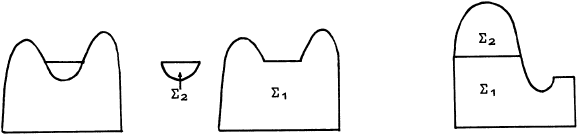
\includegraphics[scale=0.6]{suma}
\caption{Diferencia y suma respectivamente.}
\end{figure}

\section{Contornos}

 Si $\Sigma\subset\R^3$ es una esfera encerrando una bola cerrada $\overline{\Sigma}$. Definimos su \emph{contorno} como $C(\Sigma)$, el espacio cociente $\overline{\Sigma}/\sim$ de la relación $x\sim y$ si hay un segmento vertical contenido en $\overline{\Sigma}$ uniendo $x$ e $y$. En otras palabras, $C(\Sigma)$ es el espacio de hojas de la foliación de $\overline{\Sigma}$ mediante líneas verticales. La aplicación cociente se denotará $C:\overline{\Sigma}\to C(\Sigma)$. Nótese que $C$ restringida a $\Sigma$ es sobreyectiva. 
 

Vemos en la figura \ref{contorno} una esfera primitiva, cuyo contorno es un disco con una ``lengua''.


 

Motivados por esta construcción damos las siguientes definiciones.
 \begin{defi}
 Sean $n$ funciones de clase $C^1$, $f_1,\dots, f_n:[0,1]\to\R$ nulas en el borde y verificando que si $f_i(x)=f_j(x)$ para algún $x\in [0,1]$ entonces $f_i'(x)=f_j'(x)$. La figura formada por sus grafos se llamará \emph{bloque de bigones}. Un \emph{sistema de bigones} es una unión finita de bloques disjuntos. Para $n=2$, la adherencia de la unión de las componentes acotadas se llama una \emph{lengua}. 
 \end{defi}
 
 \begin{figure}[h!]
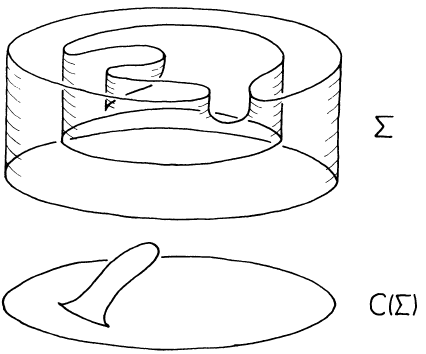
\includegraphics[scale=0.5]{contorno}
\caption{Contorno de una esfera primitiva.}\label{contorno}
\end{figure}

\begin{defi}\label{lenguas}
Una \emph{estructura de lenguas} $\mathcal{L}$ es una superficie con borde $L$, dotada de una proyección $\pi:L\to\R^2$, un disco inicial $D_0$ y una colección finita de lenguas $T_1,\dots, T_n$ sobre $L$ con las condiciones siguientes:
\begin{enumerate}
\item $L$ es unión de discos lisos $D_1,\dots, D_n$ con $D_0$, tales que sobre cada interior de los cuales $\pi$ es una sumersión. 
\item $\pi(D_i)\cap\pi\left(\bigcup_{j<i}D_j\right)$ es un subdisco $d_i$ de $\pi(D_i)$ tal que $d_i\cap\pi(D_i)$ contiene al menos un arco. 
\item $T_i=adh(\pi(D_i)-d_i)$, $int(T_i)\cap int(T_j)=\emptyset$ y $D_0\cap int(T_i)=\emptyset$. El lado de unión de $T_i$ es $T_i\cap d_i$ y su lado libre es $adh(\partial T_i-\partial d_i)$. 
\item Todo punto del lado de unión pertenece al lado libre de alguna otra lengua o a $\partial D_0$.  
\end{enumerate}
\end{defi}

Una lengua no tiene por qué ser conexa, por ello podemos hablar de \emph{subdivisión} de una estructura de lenguas, en la que se eligen como lenguas distintas algunas de las componentes de una lengua existente. 

\begin{teorema}(\cite[3.3]{Bo})
Si $\Sigma$ es una esfera primitiva, el contorno $C(\Sigma)$ admite una estructura de lenguas. 
\end{teorema}

\begin{figure}[h!]
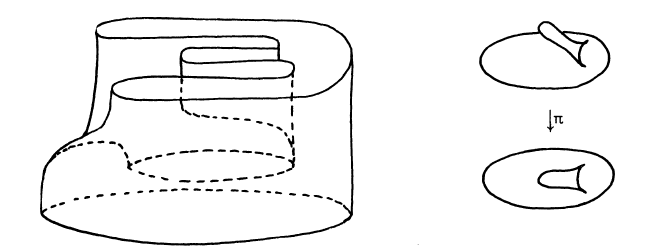
\includegraphics[scale=0.6]{contour}
\end{figure}

\begin{nota}\
\begin{enumerate}
\item La definición \ref{lenguas} se extiende a familias de esferas.
\item El orden de unión de las lenguas no forma parte de la estructura, pero para una familia se puede dar un orden localmente en el espacio de parámetros.  
\end{enumerate}
\end{nota}

Sea $\Sigma$ una esfera primitiva y $\Delta_1,\dots, \Delta_n$ una colección de discos de cirugía en planos horizontales distintos, con $int(\Delta_i)\cap\Sigma=\emptyset$. Tenemos $\Sigma\cup\Delta_1\cup\cdots\cup\Delta_n$ como unión de factores $\Sigma_0\cup\cdots\cup \Sigma_n$ con $\Delta_k$ cara de $\Sigma_k$ para $k\geq 1$. Suponemos que $\Sigma_0$ es \emph{grande}, esto es, que $\pi(\Sigma_0)\cap\partial\Sigma$ contiene un arco. Para una familia $\Sigma_t$ pedimos que $\pi(\Sigma_{0t})\cap\partial\Sigma_t$ contenga localmente arcos que varíen suavemente con $t$.

\begin{teorema}(de compatibilidad, \cite[Proposición 5.2]{Ha})
Existe una estructura de lenguas $\mathcal{L}$ (resp. $\mathcal{L}_i$) sobre $C(\Sigma)$ (resp. $\Sigma_i$) verificando las condiciones siguientes:
\begin{enumerate}
\item Para $k\geq 1$, $C(\Delta_k)$ es el disco inicial de $\mathcal{L}_k$. El disco inicial $D_0$ de $\mathcal{L}_0$ es también disco inicial de $\mathcal{L}$.
\item La unión de los $\pi(\partial T_i)$ es un sistema de bigones.
\item Para $j\neq j'$, $int(T_j)\cap int(T_{j'})=\emptyset$ o bien hay una relación de contención. 
\end{enumerate}
\end{teorema}

En presencia de un parámetro el enunciado es el mismo salvo que el factor inicial $\Sigma_{0t}$ no puede ser seguido continuamente en general. Por ejemplo si tomamos como factor inicial uno tal que la proyección tenga la forma de la figura siguiente y hacemos que varíe hasta que la lengua deje de sobresalir.

\begin{tikzpicture}[line cap=round,line join=round,>=triangle 45,x=1.0cm,y=1.0cm]
\clip(-4.3,-1.2) rectangle (18.7,3.3);
\draw [rotate around={0.:(2.5,1.)},line width=2.pt] (2.5,1.) ellipse (2.5645005658970774cm and 2.080063256847356cm);
\draw [line width=2.pt,] (3.,2.)-- (3.,0.6);
\draw [line width=2.pt,] (3.,2.)-- (5.,2.);
\draw [line width=2.pt,] (3.,0.6)-- (5.015599314732565,0.5957315454220427);
\draw [shift={(5.007799657366283,1.2978657727110212)},line width=2.pt]  plot[domain=-1.559688284679515:1.5819043689102783,variable=\t]({1.*0.7021775471956665*cos(\t r)+0.*0.7021775471956665*sin(\t r)},{0.*0.7021775471956665*cos(\t r)+1.*0.7021775471956665*sin(\t r)});
\end{tikzpicture}

 Para arreglarlo cambiamos de factor a lo largo de una subvariedad $V$ de codimensión 1 del espacio de parámetros; a un lado el punto crítico elegimos $\Sigma_{0t}=\Sigma'_t$ y al otro lado elegimos $\Sigma_{0t}=\Sigma''_t$. Se verifica que $\Sigma'_t$ y $\Sigma''_t$ tienen una cara común de tipo suma $\Delta_t$. Si para $t\in V$ tomamos $C(\Delta_t)$ como disco inicial de $\mathcal{L}$, entonces el teorema de compatibilidad se preserva en presencia de un parámetro. 

Antes de seguir avanzando enunciamos un hecho esencial: una familia de esferas primitivas es homótopa a cero dentro del espacio de todas las esferas. Esto será establecido en la siguiente sección gracias a la estructura de contorno. En cierta forma, el problema se vuelve 2-dimensional y admite solución gracias al ``pequeño teorema de Smale'' \cite[Proposición 4.2]{Bo} $Diff(D^2\ rel\ \partial D^2)$ es contráctil. Finalmente, el teorema en dimensión 3 aparece como consecuencia del teorema en dimensión 2. 
\section{Aplastamientos}

\begin{defi}
Dada una familia de superficies $L_s$, $s\in [0,1]$, con una estructura de lenguas $\mathcal{L}_s$ verificando:
\begin{enumerate}
\item Para $s>s'$, $L_s\subset L_{s'}$ y $\mathcal{L}_s=\mathcal{L}_{s'}\cap L_s$.
\item $L_1$ es un disco. 
\end{enumerate}
Decimos entonces que una tal deformación es un \emph{aplastamiento} de $\mathcal{L}_0$, \emph{parcial} si la condición 2 no se verifica. 
\end{defi}

\begin{prop}[pequeño teorema de Smale adaptado]
El espacio de aplastamientos de una estructura de lenguas tiene el tipo de homotopía de un punto.
\end{prop}

Para explicar esta proposición, en primer lugar tengamos en cuenta que una familia de esferas primitiva da lugar a un grafo en el que los vértices se tienen puntos críticos de la función altura y las aristas conectan dos consecutivos. Se sabe que estos grafos siempre dan lugar a un árbol, por lo que la contracción de aristas se traduce en un aplastamiento de la estructura de lenguas de los contornos. 

Por otra parte, tenemos el siguiente resultado 

\begin{prop}\label{monotono}
Si $\Sigma$ es una 2-esfera cuyo contorno admite una estructura de lenguas, entonces, para todo aplastamiento $C(\Sigma)_s$, existe una familia $\Sigma_s$ con $\Sigma_0=\Sigma$ tal que:
\begin{enumerate}
\item $C(\Sigma_s)=C(\Sigma)_s$,
\item para $s>s'$, $\overline{\Sigma}_s\subset\overline{\Sigma}_{s'}$ (monotonía).
\end{enumerate} 
Además, dado el aplastamiento, el conjunto de caminos $\{\Sigma_s\}$ es contráctil. 
\end{prop}
\begin{dem}
Denotamos $C=C(\Sigma)$. Sean $T_1,\dots, T_n$ lenguas de $C$ pegadas en el orden de escritura, y sea $D$ el disco inicial de $C$. A partir del aplastamiento $C_s$ definimos una familia de discos con lenguas $C(s_0,\dots, s_n)\subset C$, para $0\leq s_0\leq\cdots\leq s_n\leq 1$, con las condiciones $C(s_0,\dots, s_n)\cap T_i=C_{s_i}\cap T_i$ y $C(s_0,\dots, s_n)\cap D=C_{s_0}\cap D$. Vemos $C(0,\dots, 0,s_i,s_{i+1},\dots, s_n)$ para $s_i\in[0,s_{i+1}]$ como un aplastamiento de $C(0,\dots, 0,s_{i+1},\dots, s_n)$. Si asumimos inductivamente que hemos construido una familia $\Sigma(0,\dots, 0, s_{i+1},\dots, s_n)$ con contorno igual a $C(0,\dots, 0,s_{i+1},\dots, s_n)$, será suficiente elevar el aplastamiento $C(0,\dots, 0,s_i,s_{i+1},\dots, s_n)$ a una isotopía de aplastamientos $\Sigma(0,\dots, 0, s_i, s_{i+1},\dots, s_n)$. Para el aplastamiento buscado, $\Sigma_s=\Sigma(s,\dots, s)$. 

Por tanto, nos reducimos a dos casos: o bien una sola lengua $T=T_i-C_{s_{i+1}}$ se está aplastando, o bien se está aplastando el disco inicial. Consideramos el primer caso, ya que el segundo es similar. Como paso previo a elevar el aplastamiento $C_s$, construimos una pequeña isotopía de aplastamientos $\Sigma'_s$ de $\Sigma=\Sigma'_0$ tal que:
\begin{enumerate}[a)]
\item $\Sigma'_s$ es suave para $s>0$. 
\item $\Sigma'_s$ no tiene tangentes verticales en puntos que se proyecten sobre $int(T)$. 
\item $C(\Sigma'_s)=C(\Sigma)$. 
\end{enumerate}
Para conseguir a) seguimos la siguiente figura:

\vspace{0.5cm}




\begin{figure}[h!]
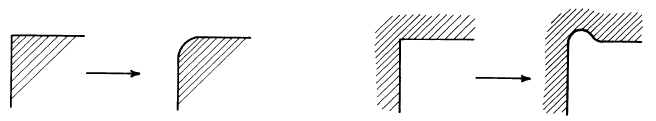
\includegraphics[scale=0.7]{(a)}
\end{figure}
Para conseguir b), sea $V$ el conjunto de puntos de $\Sigma$ que tienen plano tangente vertical y se proyectan a los puntos de $int(T)$. Sea $V_+$ (resp. $V_-$) el subconjunto de puntos donde una línea vertical hacia arriba (resp. abajo) pasa del interior de $\Sigma$ al exterior, como en la figura.

\begin{figure}[h!]
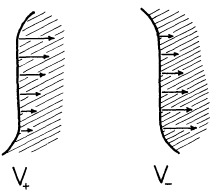
\includegraphics[scale=0.7]{vectores}
\end{figure}


 Nótese que $V_+$ y $V_-$ son disjuntos y cerrados relativos en $C^{1-}(int(T))$. Así que podemos encontrar un campo de vectores suave $v$ en $\R^3$ tal que:
\begin{enumerate}[i)]
\item $v|_{\Sigma}$ es no nulo solamente en $C^{-1}(int(T))$.
\item $v|_{\Sigma}$ es ortogonal a $\Sigma$, apuntando al interior cuando no es nulo. 
\item $\parcial{|v|}{z}>0$ en $V_+$ y $\parcial{|v|}{z}<0$ en $V_-$.
\end{enumerate}
Teniendo $v$, obtenemos $\Sigma'_s$ fluyendo con $v$ en un intervalo $[0,\varepsilon]$ lo bastante pequeño y luego permaneciendo quieto en $[\varepsilon,1]$. 

El aplastamiento de deseado $\Sigma_s$ se obtiene definiento $\overline{\Sigma}_s=C^{-1}(C_s)$.
\QED
\end{dem}

El resultado anterior también es válido en presencia de un parámetro \cite[Lema 6.1]{Ha}, luego combinándolo con el pequeño teorema de Smale, asociamos a $\Sigma$, para una estructura de lenguas fija $\mathcal{L}$ sobre $C(\Sigma)$, un conjunto contráctil de caminos monótonos (en el sentido de la proposición \ref{monotono}) $\mathcal{C}(\Sigma,\mathcal{L})$, relacionando $\Sigma$ con una esfera estándar. Esto prueba que cualquier familia de esferas primitivas es contráctil en el espacio de todas las esferas (pues admiten una estructura de lenguas). 

Si $\mathcal{L}'$ es una subdivisión de $\mathcal{L}$, entonces $\mathcal{C}(\Sigma,\mathcal{L}')\subset\mathcal{C}(\Sigma,\mathcal{L})$ como retracto de deformación, ya que ambos términos son contráctiles. 

Dada $\Delta$ una cara de $\Sigma$, denotamos $\Delta'=adh(\Sigma-\Delta)$. Supongamos que $C(\Delta)$ es el disco inicial de la estructura $\mathcal{L}$. Entonces un aplastamiento $C(\Sigma)$ sobre $C(\Delta)$ se eleva a una isotopía monónota de $\Sigma-int(\Delta)$ relativa a $\partial \Delta$, a través de $\overline{\Sigma}$ hasta $\Delta$. Lo mismo es cierto con la aparición de un parámetro. Esta isotopía se puede considerar como un conjunto de caminos de discos $\Delta_s$, $\mathcal{C}(\Sigma,\mathcal{L},\Delta)$, que se inyecta en $\mathcal{C}(\Sigma,\mathcal{L})$ como retracto de deformación mediante $\Delta_s\mapsto \Sigma_s$.

\subsection{Compatibilidad con la suma}

Sea $\Sigma$ una esfera primitiva y $\Delta$ un disco de cirugía de tipo suma, de modo que $\overline{\Sigma}=\overline{\Sigma}_0\cup\overline{\Sigma}_1$. Se tienen aplicaciones naturales $C(\Sigma_i)\to C(\Sigma)$ gracias a que $\Sigma_0$ es grande. Las estructuras de lenguas son $\LL,$ $\LL_0$ y $\LL_1$. El aplastamiento de $C(\Sigma_1)$ sobre $C(\Delta)$ da un aplastamiento parcial de $C(\Sigma)$ que se eleva a un camino monótono entre $\Sigma$ y $\Sigma_0$. Por tanto:
\begin{prop}
A todo camino $\gamma\in\mathcal{C}(\Sigma_1,\mathcal{L}_1,\Delta)$ se le puede asociar continuamente una deformación de $\CC(\Sigma_0,\LL_0)$ hasta un retracto de deformación de $\CC(\Sigma,\LL)$. 
\end{prop}

\subsection{Compatibilidad con la diferencia}

Ahora, $\overline{\Sigma}_0$ contiene a $\overline{\Sigma}_1$ y a $\overline{\Sigma}=adh(\overline{\Sigma}_0-\overline{\Sigma}_1)$. El aplastamiento de $C(\Sigma_1)$ no tiene en general el efecto de aplasta $C(\Sigma)$, sino que pueden surgir más lenguas. Incluso puede ocurrir que $C(\Sigma)$ no tenga una estructura de lenguas \cite[Sección 7]{Ha}. Para una subdivisión adecuada $\LL_1'$ de $\LL_1$ se demuestra lo siguiente \cite[Secciones 10 y 11]{Ha} sea $\Delta'=adh(\Sigma_1-\Delta)$ y sea $\{\Delta'(s)\}\in\CC(\Sigma_1,\LL_1',\Delta)$. Nótese que $\Sigma(s)=(\Sigma-\Delta')\cup\Delta'(s)$. Entonces $C(\Sigma(s))$ posee una estructura de lenguas. Por tanto podemos obtener:
  \begin{prop}
  A todo camino $\gamma\in\CC(\Sigma_1,\LL_1,\Delta)$ se le puede asociar una deformación de $\CC(\Sigma,\LL)$ hasta un retracto de deformación de $\CC(\Sigma_0,\LL_0)$. 
  \end{prop}
  
  \begin{figure}[h!]
  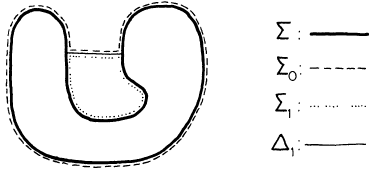
\includegraphics[scale=0.7]{ejemplo}
  \caption{Ejemplo en el que el aplastamiento de un factor no es compatible con el aplastamiento de la diferencia.}
  \end{figure}
  
En presencia de un parámetro, $\LL_1'$ no puede ser seguido de forma continua en general, pues ocurre una bifurcación donde $\LL_1'$ debe ser subdividida. 

\section{Cómo hacer continua la familia $\Sigma_{to}$}

La continuidad de la que se trata es en el sentido $C^1$ de Hausdorff: si $\Delta$ es la cara de $\Sigma_{t0}$ existente para $t\in X_{il}$, esta se desdobla en dos discos vecinos cuando la coordenada transversal $t_{il}<0$ (proceso continuo) hasta que desaparece para $t_{il}>0$ (discontinuidad).

\subsection{Orden en las caras}

En un factor inicial elegido en una componente de $\Sigma_{t0}$ existe un orden parcial natural entre sus caras $\Delta_1,\dots, \Delta_n$: $\Delta_j>\Delta_i$ si todo camino de $\Sigma_{t0}$ que tenga a $\Delta_j$ como factor inicial corta $\Delta_i$.

\subsection{Conclusión}


\section{Prueba de la conjetura de Smale}

\addcontentsline{toc}{chapter}{Bibliografía}
\begin{thebibliography}{}
\bibitem{Ha}
\bibitem{Bo}
\bibitem{Se} https://pdfs.semanticscholar.org/e737/a4f8b93242910c050c2faf761236dcf60f64.pdf
\end{thebibliography}



\end{document}